%%======================================================================
%% A template for master's/doctoral thesis. (Shivam Garg, 2021)
%%----------------------------------------------------------------------
%% As far as I'm aware, it satisfies the requirements given in https://www.ualberta.ca/graduate-studies/media-library/current-students/academicrequirements/thesisrequirementandpreparation/2016-03-29-fgsrminimumthesisformattingrequirements.pdf.
%% 
%% Might not work with an old LaTeX version. I used it successfully with TeX Live 2021 on Ubuntu. (Overleaf always has the latest version.)
%%
%% A thesis created using this template is available here: https://svmgrg.github.io/documents/alternate_estimator_thesis_2021.pdf.
%%======================================================================

%%======================================================================
%% For PDF/A conversion (file meta-data)
%%----------------------------------------------------------------------
\begin{filecontents*}[overwrite]{\jobname.xmpdata}
  \Title{Title of your thesis}
  \Author{Author name}
  \Language{en-US}
  \Subject{Computing Science}
\end{filecontents*}
%%----------------------------------------------------------------------

\RequirePackage[hyphens]{url}
\documentclass[letter, 11pt]{report}

%%======================================================================
%% For PDF/A conversion (https://webpages.tuni.fi/latex/pdfa-guide.pdf)
%%----------------------------------------------------------------------
\usepackage[utf8]{inputenc}
\usepackage[USenglish]{babel}
\usepackage{colorprofiles}
\usepackage[a-3b,mathxmp]{pdfx}[2018/12/22]
\hypersetup{pdfstartview=}
%%----------------------------------------------------------------------

\usepackage{fullpage}
\usepackage{titling}
\usepackage{graphicx}
\usepackage{nicefrac}
\usepackage{xcolor}
\usepackage{amsmath}
\usepackage{amssymb}
\usepackage{amsthm}
\PassOptionsToPackage{hyphens}{url}
\usepackage{hyperref}
%% https://tex.stackexchange.com/questions/823/remove-ugly-borders-around-clickable-cross-references-and-hyperlinks
%% \usepackage[hidelinks]{hyperref}
\hypersetup{
  colorlinks,
  linkcolor={red!33!black},
  citecolor={blue!33!black},
  urlcolor={blue!33!black}
}
% \usepackage{IEEEtrantools} %% uncomment if you use this environment
\usepackage{bbm}
\usepackage{lineno}
\usepackage{multirow}
\usepackage{longtable}
\usepackage{makecell}
\usepackage{lipsum}
\usepackage{etoolbox} %% <- for \pretocmd and \apptocmd
\usepackage{algorithm}
\usepackage[noend]{algpseudocode}
\usepackage[normalem]{ulem}
\usepackage{setspace}
\usepackage{thmtools, thm-restate}
\usepackage[nottoc]{tocbibind} % for adding list of figures to the table of contents

\setlength{\droptitle}{-6em}   % This is your set screw, for shifting up the title
\renewcommand{\baselinestretch}{1.1}
\setlength{\parskip}{0.5em}

\makeatletter %% <- make @ usable in macro names
\newcommand*\linenomathpatch{\@ifstar{\linenomathpatch@AMS}{\linenomathpatch@}}
\newcommand*\linenomathpatch@[1]{
  \expandafter\pretocmd\csname #1\endcsname {\linenomathWithnumbers}{}{}
  \expandafter\pretocmd\csname #1*\endcsname{\linenomathWithnumbers}{}{}
  \expandafter\apptocmd\csname end#1\endcsname {\endlinenomath}{}{}
  \expandafter\apptocmd\csname end#1*\endcsname{\endlinenomath}{}{}
}
\newcommand*\linenomathpatch@AMS[1]{
  \expandafter\pretocmd\csname #1\endcsname {\linenomathWithnumbersAMS}{}{}
  \expandafter\pretocmd\csname #1*\endcsname{\linenomathWithnumbersAMS}{}{}
  \expandafter\apptocmd\csname end#1\endcsname {\endlinenomath}{}{}
  \expandafter\apptocmd\csname end#1*\endcsname{\endlinenomath}{}{}
}
\let\linenomathWithnumbersAMS\linenomathWithnumbers
\patchcmd\linenomathWithnumbersAMS{\advance\postdisplaypenalty\linenopenalty}{}{}{}
\makeatother %% revert @
% \linenomathpatch{IEEEeqnarray} %% uncomment if you use IEEEeqnarray
\linenomathpatch{equation}
\linenomathpatch*{gather}
\linenomathpatch*{multline}
\linenomathpatch*{align}
\linenomathpatch*{alignat}
\linenomathpatch*{flalign}

\declaretheorem{theorem}
\newtheorem{prop}{Proposition}
\newtheorem{thm}{Theorem}
\newtheorem{eg}{Example}
\newtheorem{cor}{Corollary}[prop]
\newtheorem{lemma}{Lemma}[prop]

%%======================================================================
%% Define extra things such as the math symbols here.
%%----------------------------------------------------------------------
\DeclareMathOperator{\E}{\mathbb{E}}
\DeclareMathOperator{\V}{\mathbb{V}}

\DeclareMathOperator{\avec}{\bf a}

\DeclareMathOperator{\thetavec}{\boldsymbol{\theta}}
%%----------------------------------------------------------------------

\begin{document}

\setcounter{page}{1}
\renewcommand{\thepage}{\roman{page}} % Roman numerals for page counter

\begin{titlepage}
  \centering
  \textbf{\large{Title of your thesis}}
  \vskip.5in by \vskip.5in
  \large{Author name}

  \vfill \vfill
  A thesis submitted in partial fulfillment of the requirements for the degree of
  \vskip.3in Master of Science 
  \vskip.3in \vfill \vfill
  Department of Computing Science
  \vskip.3in
  University of Alberta
  \vfill \vfill
  $\copyright$ Author name, 2021
\end{titlepage}

% \linenumbers %% uncomment if you want to have line numbers (for review)

\doublespacing

\chapter*{Abstract} \addcontentsline{toc}{chapter}{Abstract}
Add the abstract here.

\setcounter{page}{2}
\renewcommand{\thepage}{\roman{page}} % Roman numerals for page counter

\onehalfspacing
\chapter*{Preface} \addcontentsline{toc}{chapter}{Preface}
Add the preface here.

\chapter*{Acknowledgements} \addcontentsline{toc}{chapter}{Acknowledgements}
Add ack here.

\tableofcontents
\listoftables
\listoffigures
\listofalgorithms \addcontentsline{toc}{chapter}{List of Algorithms}

\chapter{Introduction} \label{sec: introduction}

\setcounter{page}{1}
\renewcommand{\thepage}{\arabic{page}} % arabic numerals for page counter

Start introduction from here.\footnote{Writing help is available here: \url{https://terrytao.wordpress.com/advice-on-writing-papers/}.}

\section{This is the First Section}
Contents...

\begin{figure}[!hbp]
  \centering
  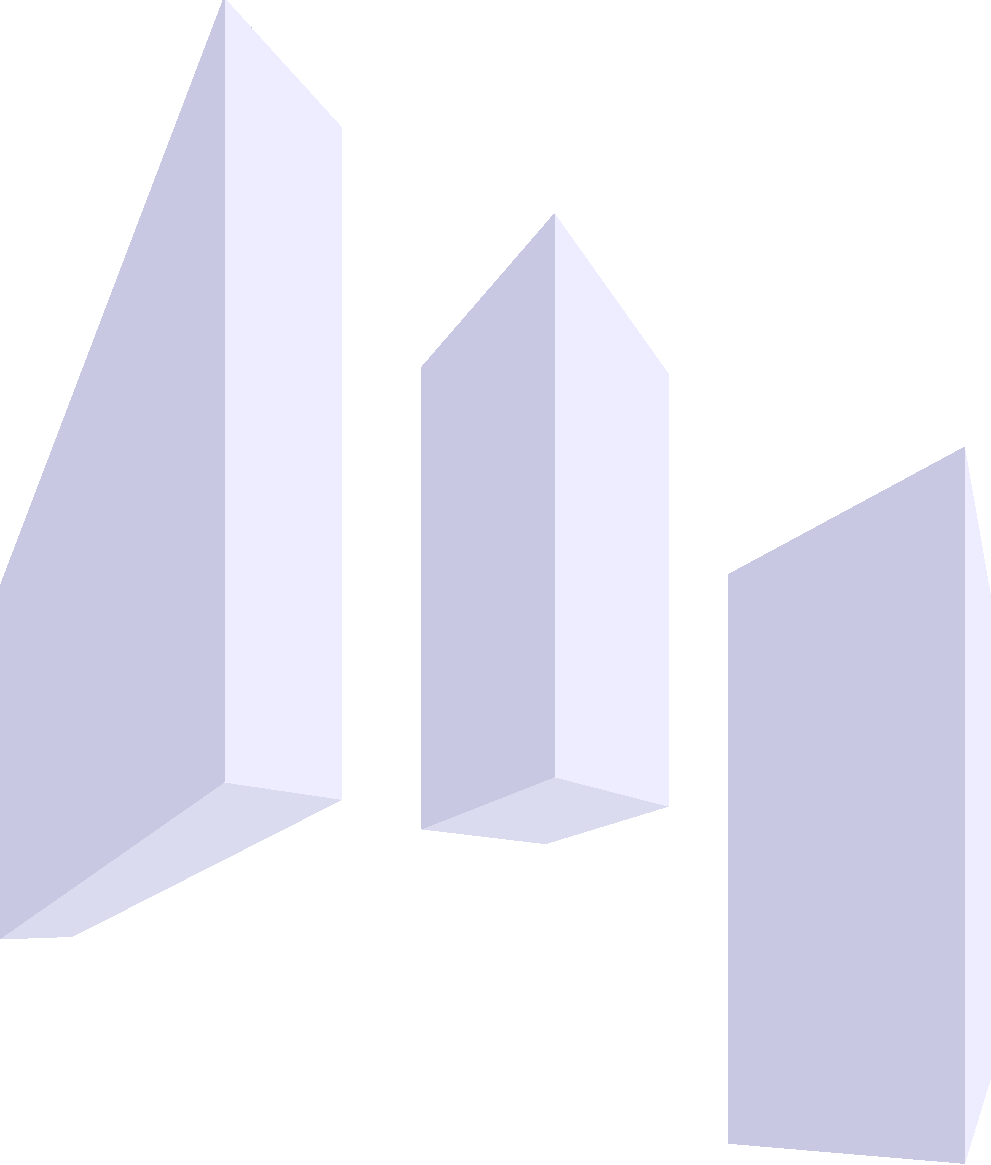
\includegraphics[scale=0.4]{figures/drawing.pdf}
  \caption{Figure caption.} 
  \label{fig: figure_name}
\end{figure}

\begin{algorithm}[!hbt]
  \caption{Algorithm caption.}
  \label{alg: alg_name}
  \begin{algorithmic}
    \State Pseudocode line 1
    \State Pseudocode line 2
  \end{algorithmic}
\end{algorithm}

\begin{restatable}{thm}{thm_name} \label{thm: thm_name}
  Theorem statement.
\end{restatable}
\begin{proof}
  Add the proof here.
\end{proof}

\begin{table}[!hbt]
  \centering
  \begin{tabular}{c|c|c}
    \textbf{Col 1}& \textbf{Col 2} & \textbf{Col 3} \\
    \hline \hline
    text & text & text \\
    \hline
    text & text & text \\
  \end{tabular}
  \caption{Table caption.} 
  \label{table: caption}
\end{table}

\section{This is the Second Section}
Contents...

\chapter{Another Chapter} \label{sec: another_chap}
If you wish to, you can also use a separate \texttt{.tex} file for each chapter, and then include a reference to that file here.

%% Following uses manually added references. If you prefer, replace this with BibTeX.
% \chapter*{References}
% \addcontentsline{toc}{chapter}{References}

% \medskip
% %% \small

% \begin{list}{}{%
%     \setlength{\topsep}{0pt}%
%     \setlength{\leftmargin}{0.2in}%
%     \setlength{\listparindent}{-0.2in}%
%     \setlength{\itemindent}{-0.2in}%
%     \setlength{\parsep}{\parskip}%
%   }%
  
% \item[] Einstein, A., Newton, I., Feynman R.P. (2002). Lectures on the unified theory of physics. \textit{Physical Review, 92}(5), 1324.
  
% \item[] Einstein, A., Newton, I., Feynman R.P. (2003). More lectures on the unified theory of physics. \textit{Physical Review, 99}(3), 1324.
% \end{list}

This is an example reference \cite{sorg2010linear}.

\renewcommand{\bibname}{References}
\bibliography{ref}
\bibliographystyle{alpha}

\end{document}
